\documentclass[11pt,a4paper]{report}
\usepackage[spanish,es-nodecimaldot]{babel}	% Utilizar español
\usepackage[utf8]{inputenc}					% Caracteres UTF-8
\usepackage{graphicx}						% Imagenes
\usepackage[hidelinks]{hyperref}			% Poner enlaces sin marcarlos en rojo
\usepackage{fancyhdr}						% Modificar encabezados y pies de pagina
\usepackage{float}							% Insertar figuras
\usepackage[textwidth=390pt]{geometry}		% Anchura de la pagina
\usepackage[nottoc]{tocbibind}				% Referencias (no incluir num pagina indice en Indice)
\usepackage{enumitem}						% Permitir enumerate con distintos simbolos
\usepackage[T1]{fontenc}					% Usar textsc en sections
\usepackage{amsmath}				% Símbolos matemáticos
\usepackage{listings}
\usepackage{color}

 
\definecolor{codegreen}{rgb}{0,0.6,0}
\definecolor{codegray}{rgb}{0.5,0.5,0.5}
\definecolor{codepurple}{rgb}{0.58,0,0.82}
\definecolor{backcolour}{rgb}{0.95,0.95,0.95}
 
\lstdefinestyle{mystyle}{
    backgroundcolor=\color{backcolour},   
    commentstyle=\color{codegreen},
    keywordstyle=\color{magenta},
    numberstyle=\tiny\color{codegray},
    stringstyle=\color{codepurple},
    basicstyle=\footnotesize,
    breakatwhitespace=false,         
    breaklines=true,                 
    captionpos=b,                    
    keepspaces=true,                 
    numbers=left,                    
    numbersep=5pt,                  
    showspaces=false,                
    showstringspaces=false,
    showtabs=false,                  
    tabsize=2
}
 
\lstset{style=mystyle, language=C++}

% Comando para poner el nombre de la asignatura
\newcommand{\asignatura}{Simulación de Sistemas}
\newcommand{\autor}{José María Sánchez Guerrero}
\newcommand{\titulo}{Práctica 3}
\newcommand{\subtitulo}{Modelos de Simulación Dinámicos y Discretos}

% Configuracion de encabezados y pies de pagina
\pagestyle{fancy}
\lhead{\autor{}}
\rhead{\asignatura{}}
\lfoot{Grado en Ingeniería Informática}
\cfoot{}
\rfoot{\thepage}
\renewcommand{\headrulewidth}{0.4pt}		% Linea cabeza de pagina
\renewcommand{\footrulewidth}{0.4pt}		% Linea pie de pagina

\begin{document}
\pagenumbering{gobble}

% Pagina de titulo
\begin{titlepage}

\begin{minipage}{\textwidth}

\centering

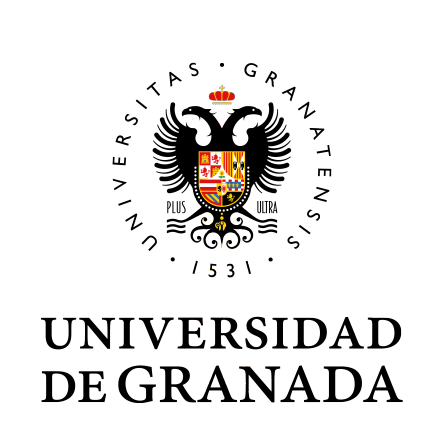
\includegraphics[scale=0.5]{img/ugr.png}\\

\textsc{\Large \asignatura{}\\[0.2cm]}
\textsc{GRADO EN INGENIERÍA INFORMÁTICA}\\[1cm]

\noindent\rule[-1ex]{\textwidth}{1pt}\\[1.5ex]
\textsc{{\Huge \titulo\\[0.5ex]}}
\textsc{{\Large \subtitulo\\}}
\noindent\rule[-1ex]{\textwidth}{2pt}\\[3.5ex]

\end{minipage}

\vspace{0.5cm}

\begin{minipage}{\textwidth}

\centering

\textbf{Autor}\\ {\autor{}}\\[2.5ex]
\textbf{Rama}\\ {Computación y Sistemas Inteligentes}\\[2.5ex]
\vspace{0.3cm}


\includegraphics[scale=0.3]{img/etsiit.jpeg}

\vspace{0.7cm}
\textsc{Escuela Técnica Superior de Ingenierías Informática y de Telecomunicación}\\
\vspace{1cm}
\textsc{Curso 2019-2020}
\end{minipage}
\end{titlepage}

\pagenumbering{arabic}
\tableofcontents
\thispagestyle{empty}				% No usar estilo en la pagina de indice

\newpage

\setlength{\parskip}{1em}

\chapter{Mi segundo modelo de simulación Discreto}

Nuestro modelo de simulación consistirá en un servidor que presta un determinado servicio a una serie de clientes, los cuales solicitarán dicho servicio
periódicamente. Cuando llega un cliente y el servidor no está ocupado, será atendido inmediatamente; en caso contrario, el cliente tendrá que esperar en
la cola. Cuando se completa un servicio, el servidor elegirá al siguiente en una forma FIFO.

Al empezar la simulación, no habrá clientes esperando y el servidor está libre. Utilizaremos el mismo generador exponencial tanto para el tiempo que tardarán
en llegar los clientes, como el tiempo que tardará el servidor en atender a cada uno.


\section{Simulación con incremento fijo de tiempo}

En esta simulación, vamos a tratar al tiempo incrementándolo de unidad en unidad. Para evitar problemas con el manejo del tiempo, tendremos que modificar
los generadores de datos para que nos devuelvan los valores redondeados al entero más próximo. Si obtenemos un valor igual a 0, devolveremos 1 en su lugar,
ya que el suceso generado quedaría en un tiempo anterior al actual, que generamos al incrementar en una unidad.

Este será nuestro código resultante, que nos servirá tanto para generar el tiempo de llegada del cliente como para generar el timepo del servicio (sólo
tendremos que modificar la variable $tlleg$ por $tserv$):
\newpage
\begin{lstlisting}
float generallegada(float tlleg){
	float u = random();         // o tambien rand() en lugar de random()
	u = ( u / (RAND_MAX+1.0) ); //RAND_MAX es una constante del sistema
	u = round( -tlleg * log(1-u) );

	if (u != 0)
		return u;
	else
		return 1.0;
}
\end{lstlisting}


Para la simulación vamos a emplear diferentes unidades de medida de tiempo (horas, minutos, segundos...) y con un número de clientes a atender bastante alto,
de unos 10.000, para que los resultados sean robustos. Este es el resultado que obtenemos:
\begin{table}[H]
\resizebox{\textwidth}{!}{%
\begin{tabular}{c|c|c|c|c}
\textbf{tiempo} & \textbf{tlleg} & \textbf{tserv} & \textbf{\% tiempo ocioso} & \textbf{Media clientes en cola} \\ \hline
horas           & 0.15           & 0.1            & 0.019994                  & 0.000000                        \\ \hline
medias horas    & 0.3            & 0.2            & 0.625621                  & 0.078153                        \\ \hline
cuartos de hora & 0.6            & 0.4            & 7.224885                  & 0.356633                        \\ \hline
minutos         & 9              & 6              & 31.501728                 & 1.647961                        \\ \hline
segundos        & 540            & 360            & 33.934223                 & 1.282934                        \\
\end{tabular}%
}
\end{table}

Como podemos ver, los porcentajes de tiempo ocioso del servidor tienen una variación bastante grande. Esto se debe a que los valores pequeños (unidades de tiempo
más altas como las horas o la medias horas) producen unos valores muy próximos a cero en los generadores y, en consecuencia, son redondeados. Como ya hemos visto,
estos valores no serán devueltos como 0, si no como 1.

Con esto estamos diciendo que un suceso dura más de lo que realmente es, y vamos acumulando este error en toda la simulación. Esta es la razón por la cual los
modelos de incremento fijo no son los más apropiados, ya que sus valores son bastante diferentes a los que obtendríamos sobre el papel.

A continuación, vamos a mostrar unas gráficas con diversas ejecuciones para comprobar que los resultados obtenidos son coherentes y ver mejor las diferencias que
obtenemos al utilizar distintas medidas tiempo:
\begin{figure}[H]
\centering
\begin{minipage}{0.5\textwidth}
  \centering
  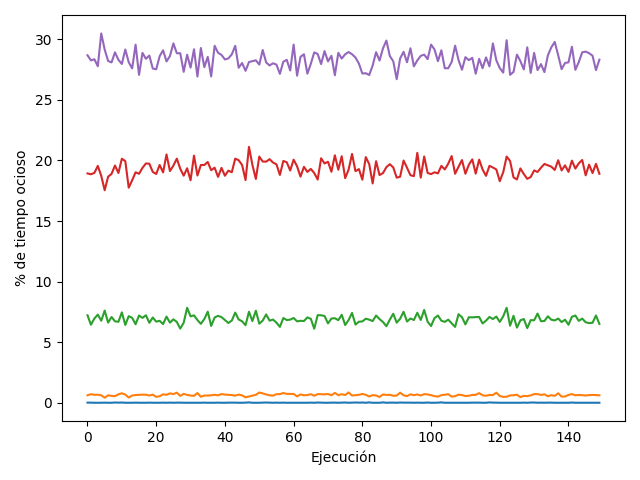
\includegraphics[scale=0.4]{img/incremento-fijo-ocioso.png}
\end{minipage}%
\begin{minipage}{0.5\textwidth}
  \centering
  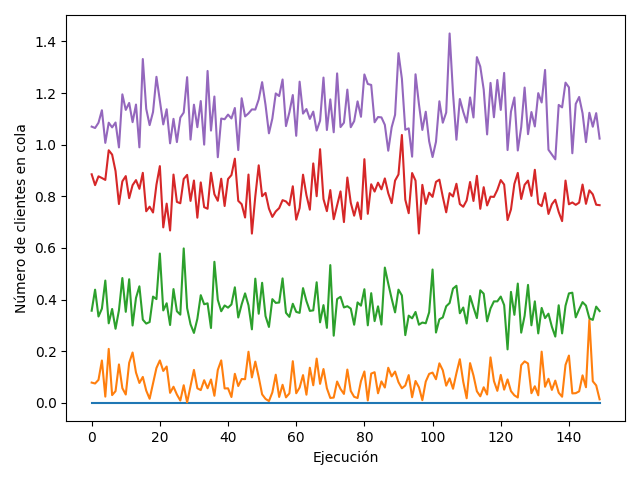
\includegraphics[scale=0.4]{img/incremento-fijo-cola.png}
\end{minipage}
\caption{Porcentaje de tiempo ocioso del servidor y media de clientes en cola}
\end{figure}

Aqui podemos observa cómo las gráficas van teniendo un porcentaje de ocupación y un número de clientes en cola más alto a medida que disminuimos las valores $tlleg$
y $tserv$. También podemos observar que, pese a que cada una de las líneas rondan un rango de valores, existe cierta variabilidad en los resultados; por lo cual sería
un poco irresponsable fiarnos de un solo dato como el de la tabla.


\section{Simulación con incremento variable de tiempo}

Ahora vamos a tratar el mismo problema pero con un incremento de tiempo variable, para hacerlo más eficiente y preciso. En este caso, la variable no tendrá ni por
qué ser un entero ni tendremos que parsear los generadores de datos, ya que se incrementará su valor hasta el suceso más cercano. Decimos que es más preciso porque
porque no tiene que dar los saltos que daba el anterior modelo y, en consecuencia, gana en eficiencia ya que va suceso a suceso.

Esta es la nueva línea de código que tendremos que añadir (también quitaremos la que aumenta el tiempo de manera uniforme $reloj++$):
\begin{lstlisting}
reloj = min(tiempo_llegada,tiempo_salida)
\end{lstlisting}

A continuación, vamos a ejecutar este modelo de la misma forma que hemos hecho con el modelo anterior y óbservar los cambios que se obtienen:

\begin{table}[H]
\resizebox{\textwidth}{!}{%
\begin{tabular}{c|c|c|c|c}
\textbf{tiempo} & \textbf{tlleg} & \textbf{tserv} & \textbf{\% tiempo ocioso} & \textbf{Media clientes en cola} \\ \hline
horas           & 0.15           & 0.1            & 33.993752                 & 1.260754                        \\ \hline
medias horas    & 0.3            & 0.2            & 33.555038                 & 1.250663                        \\ \hline
cuartos de hora & 0.6            & 0.4            & 34.353592                 & 1.382941                        \\ \hline
minutos         & 9              & 6              & 34.451107                 & 1.211860                        \\ \hline
segundos        & 540            & 360            & 33.695103                 & 1.261086                        \\
\end{tabular}%
}
\end{table}

Vemos que los resultados esta vez han sido más regulares, ya que para todas las medidas de tiempo se han obtenido unos valores entre el 33 y el 34 por ciento. A
diferencia del modelo anterior, en este podríamos decir que los resultados son bastante más fiables independientemente de si utilizamos horas, minutos, segundos...
Esto es debido a que ahora no tenemos la acumulación del error que teníamos anteriormente, y los sucesos se producen siempre en el momento declarado, sin ponderar.
\begin{figure}[H]
\centering
\begin{minipage}{0.5\textwidth}
  \centering
  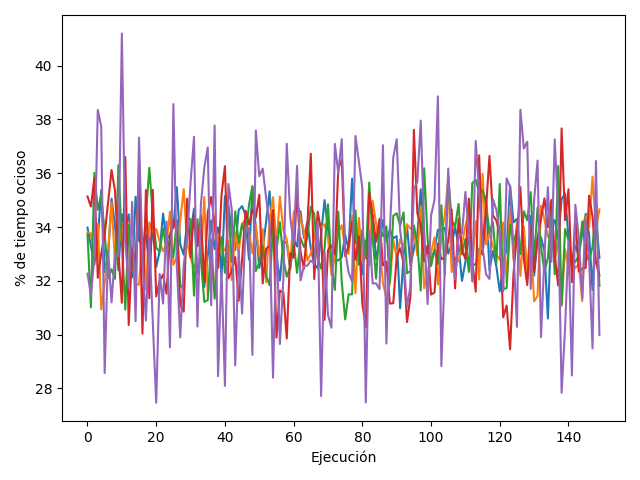
\includegraphics[scale=0.4]{img/incremento-variable-ocioso.png}
\end{minipage}%
\begin{minipage}{0.5\textwidth}
  \centering
  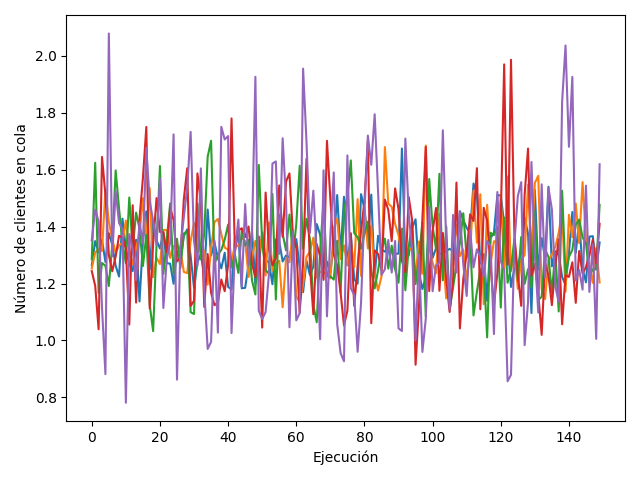
\includegraphics[scale=0.4]{img/incremento-variable-cola.png}
\end{minipage}
\caption{Porcentaje de tiempo ocioso del servidor y media de clientes en cola}
\end{figure}

Si observamos ahora las gráficas con las diversas ejecuciones, vemos que están prácticamente todas unas encima de otras. Como acabamos de decir, ya no tenemos este
error en las distintas medidas de tiempo. No obstante, vemos que aún tenemos bastante variabilidad en los datos, llegando algunos a máximos como 42 o a mínimos
como 27.

Por otra parte, esta mejora no sólo afecta a las medidas de tiempo, si no que también afecta a la eficiencia. En el modelo anterior, los incrementos en el reloj
dependen de la medida del tiempo; mientras que en el modelo actual, el número de incrementos dependerá del número de sucesos. Vamos a comprobarlo extrayendo una
tabla que compare los tiempos de ejecución para todas las medidas con incremento fijo, con las mismas medidas en incremento variable:
\begin{table}[H]
\resizebox{\textwidth}{!}{%
\begin{tabular}{c|c|c|c|c}
\textbf{tiempo} & \textbf{tlleg} & \textbf{tserv} & \textbf{tiempo fijo} & \textbf{tiempo variable} \\ \hline
horas           & 0.15           & 0.1            & 0.001671             & 0.002071                 \\ \hline
medias horas    & 0.3            & 0.2            & 0.002937             & 0.002562                 \\ \hline
cuartos de hora & 0.6            & 0.4            & 0.003491             & 0.001119                 \\ \hline
minutos         & 9              & 6              & 0.003358             & 0.001464                 \\ \hline
segundos        & 540            & 360            & 0.020543             & 0.002939                 \\
\end{tabular}%
}
\end{table}

Podemos ver que el tiempo de ejecución en el modelo con incremento fijo va aumentando lo que parece lineal o exponencialemente, mientras que en el modelo con
incremento variable tenemos unos tiempos prácticamente iguales en unas ejecuciones y otras.

\begin{figure}[H]
\centering
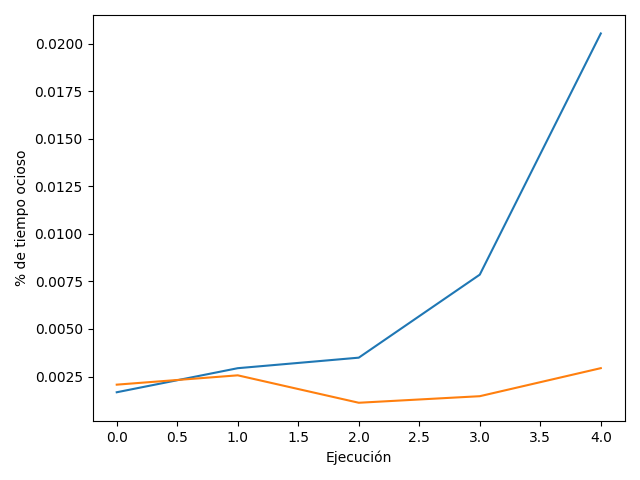
\includegraphics[scale=0.7]{img/tiempos.png}
\caption{En azul los tiempos con incremento fijo y, en naranja, variable.}
\end{figure}

En la gráfica lo podemos corroborar. Tras estudiar los dos modelos, concluímos que utilizar uno de incremento variable sería lo acertado, no sólo por la mayor
eficiencia en tiempo que nos da, si no por algo más importante como es la precisión y calidad al trabajar con distintos tipos de datos o unidades de medida.




\section{Programa de simulación dinámico y discreto}

En esta sección vamos a abordar un problema similar al anterior, pero con una cantidad de $m$ servidores idénticos trabajando en paralelo. La cola de clientes
seguirá siendo la misma, tratando a los clientes del mismo método FIFO. Si utilizamos más de un servidor en complicado, pero con $m=1$ es posible obtener los
valores teóricos de casi todas las medidas de rendimiento.

Vamos a ejecutar el programa para ver qué resultamos obtenemos. Lo haremos con unos parámetros como los anteriores ($parada=10.000$, $tlleg=9$ y $tserv=6$):
\begin{figure}[H]
\centering
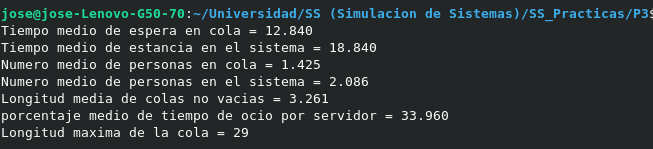
\includegraphics[scale=0.8]{img/cola-m1.png}
\caption{Ejecución del programa colammk con $m=1$.}
\end{figure}

Una vez obtenidos estos valores, vamos a contrastarlos con los teóricos. Lo primero es calcularlos:

\begin{itemize}[label=\textbullet]
	\item Tiempo medio de espera en cola
		  $= \frac{tserv^2}{tlleg-tserv} = \frac{6^2}{9-6} = \frac{36}{3} = 12$
	\item Tiempo medio de estancia en el sistema
		  $= \frac{tserv \cdot tlleg}{tlleg-tserv} = \frac{6 \cdot 9}{9-6} = \frac{54}{3} = 18$
	\item Número medio de clientes en cola
		  $= \frac{tserv^2}{tlleg (tlleg-tserv)} = \frac{6^2}{9\cdot (9-6)} = \frac{36}{27} = 1.3$
	\item Número medio de clientes en el sistema
		  $= \frac{tserv}{tlleg-tserv} = \frac{6}{9-6} = \frac{6}{3} = 2$
	\item Longitud media de colas no vacías
		  $= \frac{tlleg}{tlleg-tserv} = \frac{9}{9-6} = \frac{9}{3} = 3$
	\item Porcentaje de tiempo de ocio del servidor
		  $= \big(1 - \frac{tserv}{tlleg}\big) \cdot 100 = \big(1 - \frac{6}{9}\big) \cdot 100 = \frac{100}{3} = 33.3$
\end{itemize}

Como podemos ver, los resultados se ajustan bastante bien a los que esperábamos teóricamente. Esto se debe, en parte, a que la simulación se ha realizado con
un tiempo de parada muy alto, es decir, la simulación ha durado bastante tiempo y las medias que se obtienen son lo suficientemente representativas.

Si probamos con un tiempo de parada bajo, los resultados serán más impredecibles o variables, como se muestra a continuación:
\begin{figure}[H]
\centering
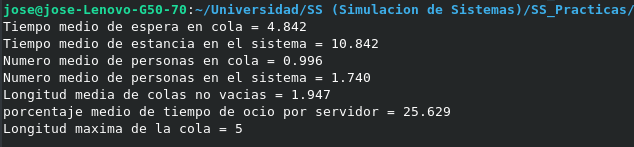
\includegraphics[scale=0.8]{img/cola2-m1.png}
\caption{Ejecución del programa colammk con $m=1$ y tiempo bajo.}
\end{figure}


Ahora vamos a aumentar el número de servidores $m$, pero manteniendo un equilibrio. El tiempo de servicio dividido por el número de servidores tiene que
permanecer constante. Vamos a modificar el programa para que repita varias veces la simulación y calcule las medias y desviaciones típicas de las medidas
de rendimiento.

Las líneas más importantes que se han modificadas son las siguientes:
\begin{lstlisting}
void fin(){
	....
	// Variables nuevas para medias y desviaciones
	retrasoMedio += retrasomedio;
	estanciaMedia += estanciamedia;
	enColaMedio += encolamedio;
	enSistemaMedia += ensistemamedio;
	colasMedia += colasnovaciasmedio;
	porcentajeOcioMedio += porcentajemedioocio;
	longMaxCola += maximacola;

	retrasoMedioDes += pow(retrasomedio, 2);
	estanciaMediaDes += pow(estanciamedia, 2);
	enColaMedioDes += pow(encolamedio, 2);
	enSistemaMedioDes += pow(ensistemamedio, 2);
	colasMediaDes += pow(colasnovaciasmedio, 2);
	porcentajeOcioMedioDes += pow(porcentajemedioocio, 2);
	longMaxColaDes += pow(maximacola, 2);
}
\end{lstlisting}
\begin{lstlisting}
float calcularDesviacion(float suma, float media)
{
    float desviacion = suma - (n_simulaciones * pow(media, 2));
    desviacion = desviacion / (n_simulaciones - 1);

    return sqrt(desviacion);
}
\end{lstlisting}

Por último ya tenemos el bucle for, la división entre el número de simulaciones para hacer la media y desviaciones típicas, y posteriormente imprimimos
los resultados.

La prueba de este programa la vamos a realizar con varios números de servidores, sin embargo, el resto de parámetros que usaremos serán los mismos que
los de la ejecución con $m=1$, ya que los resultados obtenidos eran muy similares a los valores teóricos. En este caso vamos a realizar la ejecución con
2, 3, 4 y 5 servidores, adaptando el $tserv$ a cada uno de ellos para mantener el equilibrio. Este ha sido el resultado:

\begin{table}[H]
\centering
\resizebox{\textwidth}{!}{%
\begin{tabular}{|c|c|c|c|c|}
\hline
\textbf{\begin{tabular}[c]{@{}c@{}}Número de\\ servidores\end{tabular}} & \textbf{\begin{tabular}[c]{@{}c@{}}2\\ tserv: 12\end{tabular}} & \textbf{\begin{tabular}[c]{@{}c@{}}3\\ tserv: 18\end{tabular}} & \textbf{\begin{tabular}[c]{@{}c@{}}4\\ tserv: 24\end{tabular}} & \textbf{\begin{tabular}[c]{@{}c@{}}5\\ tserv: 30\end{tabular}} \\ \hline
\textbf{\begin{tabular}[c]{@{}c@{}}Tiempo medio\\ espera en cola\end{tabular}} & \begin{tabular}[c]{@{}c@{}}med: 9.41335\\ des: 0.730856\end{tabular} & \begin{tabular}[c]{@{}c@{}}med: 7.80226\\ des: 1.19625\end{tabular} & \begin{tabular}[c]{@{}c@{}}med: 6.5818\\ des: 1.59282\end{tabular} & \begin{tabular}[c]{@{}c@{}}med: 5.78543\\ des: 0.709112\end{tabular} \\ \hline
\textbf{\begin{tabular}[c]{@{}c@{}}Tiempo medio\\ estancia en el sistema\end{tabular}} & \begin{tabular}[c]{@{}c@{}}med: 21.4133\\ des: 0.730836\end{tabular} & \begin{tabular}[c]{@{}c@{}}med: 25.8023\\ des: 1.19633\end{tabular} & \begin{tabular}[c]{@{}c@{}}med: 30.5818\\ des: 1.59289\end{tabular} & \begin{tabular}[c]{@{}c@{}}med: 35.7854\\ des: 0.70908\end{tabular} \\ \hline
\textbf{\begin{tabular}[c]{@{}c@{}}Numero medio\\ personas en cola\end{tabular}} & \begin{tabular}[c]{@{}c@{}}med: 1.05059\\ des: 0.0854933\end{tabular} & \begin{tabular}[c]{@{}c@{}}med: 0.883231\\ des: 0.0896291\end{tabular} & \begin{tabular}[c]{@{}c@{}}med: 0.746949\\ des: 0.0693109\end{tabular} & \begin{tabular}[c]{@{}c@{}}med: 0.649897\\ des: 0.0780725\end{tabular} \\ \hline
\textbf{\begin{tabular}[c]{@{}c@{}}Número medio\\ personas en el sistema\end{tabular}} & \begin{tabular}[c]{@{}c@{}}med: 2.37887\\ des: 0.0963648\end{tabular} & \begin{tabular}[c]{@{}c@{}}med: 2.87863\\ des: 0.103085\end{tabular} & \begin{tabular}[c]{@{}c@{}}med: 3.40728\\ des: 0.0925651\end{tabular} & \begin{tabular}[c]{@{}c@{}}med: 3.98036\\ des: 0.118443\end{tabular} \\ \hline
\textbf{\begin{tabular}[c]{@{}c@{}}Longitud media\\ colas no vacías\end{tabular}} & \begin{tabular}[c]{@{}c@{}}med: 2.97911\\ des: 0.172741\end{tabular} & \begin{tabular}[c]{@{}c@{}}med: 2.99961\\ des: 0.209258\end{tabular} & \begin{tabular}[c]{@{}c@{}}med: 2.98825\\ des: 0.184951\end{tabular} & \begin{tabular}[c]{@{}c@{}}med: 2.97684\\ des: 0.214132\end{tabular} \\ \hline
\textbf{\begin{tabular}[c]{@{}c@{}}Porcentaje medio\\ tiempo de ocio\end{tabular}} & \begin{tabular}[c]{@{}c@{}}med: 33.5856\\ des: 0.744918\end{tabular} & \begin{tabular}[c]{@{}c@{}}med: 33.4867\\ des: 0.718379\end{tabular} & \begin{tabular}[c]{@{}c@{}}med: 33.4917\\ des: 0.822586\end{tabular} & \begin{tabular}[c]{@{}c@{}}med: 33.3909\\ des: 1.01696\end{tabular} \\ \hline
\textbf{\begin{tabular}[c]{@{}c@{}}Longitud\\ máxima cola\end{tabular}} & \begin{tabular}[c]{@{}c@{}}med: 18.4\\ des: 3.43452\end{tabular} & \begin{tabular}[c]{@{}c@{}}med: 17.88\\ des: 3.86317\end{tabular} & \begin{tabular}[c]{@{}c@{}}med: 17.16\\ des: 3.32191\end{tabular} & \begin{tabular}[c]{@{}c@{}}med: 16.5\\ des: 2.74234\end{tabular} \\ \hline
\end{tabular}%
}
\end{table}

Podemos ver que a medida que aumentamos el número de servidores, los resultados van siendo mejores. Los tiempos medios de espera en cola se reducen, con
menos clientes en cola y, a su vez, un número mayor de clientes en el sistema.

Por otro lado, podemos ver que el porcentaje medio de tiempo de ocio del servidor es prácticamente el mismo en todos los casos (teniendo en cuenta siempre
un cierto error) y el tiempo medio de estancia en el sistema se va incrementando. Esto quiere decir que el sistema está bien equilibrado y, a su vez, deducimos
que estamos desperdiciando potencia del servidor; es decir, que pese a tener un número alto de servidores, no tenemos los suficientes clientes para que funcionen
eficientemente o, simplemente, no los distribuímos de una forma eficaz.

\newpage
Para finalizar con este modelo de simulación, vamos a estudiar que sucede si reemplzamos los generadores actuales por generadores determinísticos y uniformes.
El nuevo código implementado para el determinístico y para el uniforme, respectivamente, es:
\begin{lstlisting}
// Deterministico. Devuelve siempre el valor medio introducido
float generador_deterministico(float media)
{
	return media;
}

// Uniforme. Devuelve un valor uniformemente generado con media
// en el valor introducido
float generador_uniforme(float media)
{
	float u;
	u = (float) random();
	u = u/(float)(RAND_MAX+1.0);
	return(media*2*u);
}
\end{lstlisting}

Las pruebas también se van a hacer con una cantidad $m=1$ de servidores y con el resto de parámetros igual que en las pruebas anteriors. El resultado es el
siguiente:
\begin{table}[H]
\centering
\begin{tabular}{c|c|c}
\textbf{\begin{tabular}[c]{@{}c@{}}Tipo de\\ generador\end{tabular}} & \textbf{\begin{tabular}[c]{@{}c@{}}Generador\\ determinístico\end{tabular}} & \textbf{\begin{tabular}[c]{@{}c@{}}Generador\\ uniforme\end{tabular}} \\ \hline
\textbf{\begin{tabular}[c]{@{}c@{}}Tiempo medio\\ espera en cola\end{tabular}} & 0 & 3.498 \\ \hline
\textbf{\begin{tabular}[c]{@{}c@{}}Tiempo medio\\ estancia en el sistema\end{tabular}} & 6 & 9.498 \\ \hline
\textbf{\begin{tabular}[c]{@{}c@{}}Numero medio\\ personas en cola\end{tabular}} & 0 & 0.387 \\ \hline
\textbf{\begin{tabular}[c]{@{}c@{}}Número medio\\ personas en el sistema\end{tabular}} & 0.667 & 1.051 \\ \hline
\textbf{\begin{tabular}[c]{@{}c@{}}Longitud media\\ colas no vacías\end{tabular}} & 0 & 1.519 \\ \hline
\textbf{\begin{tabular}[c]{@{}c@{}}Porcentaje medio\\ tiempo de ocio\end{tabular}} & 33.339 & 33.534 \\ \hline
\textbf{\begin{tabular}[c]{@{}c@{}}Longitud\\ máxima cola\end{tabular}} & 0 & 6
\end{tabular}
\end{table}

Como podemos ver, el generador determinístico ha obtenido los mejores resultados posibles, con un tiempo medio de espera en la cola de 0 minutos y un tiempo
de servicio medio de 6 minutos. Esto se debe a que el generador de tiempos de servicio no produce las variaciones que se pueden dar en la vida real, y por lo
tanto, como el tiempo de llegadas es 9 minutos y el de servicio 6, nunca se pisrán el uno con el otro.

En cuanto al generador uniforme, vemos que nos da resultados diferentes a los del generador determinístico y que, en un principio, parecen bastante buenos. No
obstante, si los comparamos con los valores teóricos calculados anteriormente, vemos que son muy diferentes, lo que quiere decir que son unos valores bastante
alejados de la realidad.




\chapter{Mi tercer modelo de simulación Discreto}

En este modelo de simulación vamos a estudiar el funcionamiento de un puerto y posteriormente, realizar mejoras en el sistema para poder hacerlo más eficiente.
El puerto consta de tres puntos de atraque, por lo que podrá cargar tres petroleros simultáneamente. También tendremos tres tipos de petroleros según el tiempo
de carga que necesiten, a lo que hay que añadirle las horas que tardan los petroleros en llegar al puerto.

Tanto para atracar como para salir del puerto, cada petrolero necesitará los servicios de un remolcador. Tendremos sólo un remolcador en el puerto, el cual tarda
$1 \pm 0.25$ horas en realizar la actividad más 0.25 horas si tiene que ir desde la bocana del puerto hasta los puntos de atraque. El remolcador tratará a los
barcos de forma FIFO, tanto para los de atracan como para los que se van.

En la zona donde está situado el puerto se producen tormentas frecuentes, por lo que el remolcador quedará inactivo durante estas (excepto si ya está realizando
una actividad). Si la actividad que está viajando hasta un punto de atraque, también se cancelará la actividad.


\section{Configuración inicial del remolcador}
Haciendo uso de la implementación ya proporcionada, vamos a realizar una serie de ejecuciones con distintos números de simulaciones, para asi determinar cual
es un valor adecuado de ellas.
\begin{table}[H]
\resizebox{\textwidth}{!}{%
\begin{tabular}{|c|c|c|c|c|c|}
\hline
\textbf{\begin{tabular}[c]{@{}c@{}}Número de\\ simulaciones\end{tabular}}                          & \textbf{10}                                                              & \textbf{50}                                                              & \textbf{100}                                                             & \textbf{150}                                                             & \textbf{500}                                                             \\ \hline
\textbf{\begin{tabular}[c]{@{}c@{}}Media barcos\\ cola de llegadas\end{tabular}}                   & \begin{tabular}[c]{@{}c@{}}media: 1.333533\\ des: 0.523857\end{tabular}  & \begin{tabular}[c]{@{}c@{}}media: 1.135396\\ des: 0.411275\end{tabular}  & \begin{tabular}[c]{@{}c@{}}media: 1.166943\\ des: 0.468569\end{tabular}  & \begin{tabular}[c]{@{}c@{}}media: 1.221241\\ des: 0.439310\end{tabular}  & \begin{tabular}[c]{@{}c@{}}media: 1.201712\\ des: 0.461860\end{tabular}  \\ \hline
\textbf{\begin{tabular}[c]{@{}c@{}}Media barcos\\ cola de salidas\end{tabular}}                    & \begin{tabular}[c]{@{}c@{}}media: 0.029232\\ des: 0.004155\end{tabular}  & \begin{tabular}[c]{@{}c@{}}media: 0.028225\\ des: 0.002669\end{tabular}  & \begin{tabular}[c]{@{}c@{}}media: 0.028771\\ des: 0.003588\end{tabular}  & \begin{tabular}[c]{@{}c@{}}media: 0.028802\\ des: 0.003547\end{tabular}  & \begin{tabular}[c]{@{}c@{}}media: 0.028596\\ des: 0.003577\end{tabular}  \\ \hline
\textbf{\begin{tabular}[c]{@{}c@{}}Tiempo medio\\ puerto tipo 0\end{tabular}}                      & \begin{tabular}[c]{@{}c@{}}media: 34.803562\\ des: 5.445097\end{tabular} & \begin{tabular}[c]{@{}c@{}}media: 33.173023\\ des: 4.127820\end{tabular} & \begin{tabular}[c]{@{}c@{}}media: 33.263069\\ des: 4.946590\end{tabular} & \begin{tabular}[c]{@{}c@{}}media: 33.819340\\ des: 4.702908\end{tabular} & \begin{tabular}[c]{@{}c@{}}media: 33.678764\\ des: 4.920179\end{tabular} \\ \hline
\textbf{\begin{tabular}[c]{@{}c@{}}Tiempo medio\\ puerto tipo 1\end{tabular}}                      & \begin{tabular}[c]{@{}c@{}}media: 41.308720\\ des: 5.769780\end{tabular} & \begin{tabular}[c]{@{}c@{}}media: 38.570274\\ des: 4.494416\end{tabular} & \begin{tabular}[c]{@{}c@{}}media: 39.113869\\ des: 4.792210\end{tabular} & \begin{tabular}[c]{@{}c@{}}media: 39.822876\\ des: 4.737566\end{tabular} & \begin{tabular}[c]{@{}c@{}}media: 39.477352\\ des: 5.019176\end{tabular} \\ \hline
\textbf{\begin{tabular}[c]{@{}c@{}}Tiempo medio\\ puerto tipo 2\end{tabular}}                      & \begin{tabular}[c]{@{}c@{}}media: 52.762413\\ des: 5.920279\end{tabular} & \begin{tabular}[c]{@{}c@{}}media: 50.656128\\ des: 4.696106\end{tabular} & \begin{tabular}[c]{@{}c@{}}media: 51.064156\\ des: 5.299624\end{tabular} & \begin{tabular}[c]{@{}c@{}}media: 51.613480\\ des: 4.874365\end{tabular} & \begin{tabular}[c]{@{}c@{}}media: 51.393242\\ des: 5.082584\end{tabular} \\ \hline
\textbf{\begin{tabular}[c]{@{}c@{}}\% tiempo\\ remolcador\\ desocupado\end{tabular}}               & \begin{tabular}[c]{@{}c@{}}media: 80.564148\\ des: 0.210406\end{tabular} & \begin{tabular}[c]{@{}c@{}}media: 80.600021\\ des: 0.183851\end{tabular} & \begin{tabular}[c]{@{}c@{}}media: 80.609428\\ des: 0.160885\end{tabular} & \begin{tabular}[c]{@{}c@{}}media: 80.639183\\ des: 0.167643\end{tabular} & \begin{tabular}[c]{@{}c@{}}media: 80.619522\\ des: 0.205144\end{tabular} \\ \hline
\textbf{\begin{tabular}[c]{@{}c@{}}\% tiempo\\ remolcador\\ viajando vacío\end{tabular}}           & \begin{tabular}[c]{@{}c@{}}media: 1.170690\\ des: 0.236674\end{tabular}  & \begin{tabular}[c]{@{}c@{}}media: 1.296613\\ des: 0.218616\end{tabular}  & \begin{tabular}[c]{@{}c@{}}media: 1.309277\\ des: 0.237519\end{tabular}  & \begin{tabular}[c]{@{}c@{}}media: 1.260584\\ des: 0.239027\end{tabular}  & \begin{tabular}[c]{@{}c@{}}media: 1.272699\\ des: 0.227300\end{tabular}  \\ \hline
\textbf{\begin{tabular}[c]{@{}c@{}}\% tiempo\\ remolcador\\ remolcando\end{tabular}}               & \begin{tabular}[c]{@{}c@{}}media: 18.265163\\ des: 0.181919\end{tabular} & \begin{tabular}[c]{@{}c@{}}media: 18.103365\\ des: 0.220881\end{tabular} & \begin{tabular}[c]{@{}c@{}}media: 18.081308\\ des: 0.246783\end{tabular} & \begin{tabular}[c]{@{}c@{}}media: 18.100248\\ des: 0.256010\end{tabular} & \begin{tabular}[c]{@{}c@{}}media: 18.107714\\ des: 0.241916\end{tabular} \\ \hline
\textbf{\begin{tabular}[c]{@{}c@{}}\% tiempo puntos\\ atraque libres\end{tabular}}                 & \begin{tabular}[c]{@{}c@{}}media: 12.410981\\ des: 1.272044\end{tabular} & \begin{tabular}[c]{@{}c@{}}media: 13.255801\\ des: 1.253805\end{tabular} & \begin{tabular}[c]{@{}c@{}}media: 13.299381\\ des: 1.415099\end{tabular} & \begin{tabular}[c]{@{}c@{}}media: 13.025707\\ des: 1.442802\end{tabular} & \begin{tabular}[c]{@{}c@{}}media: 13.064457\\ des: 1.378616\end{tabular} \\ \hline
\textbf{\begin{tabular}[c]{@{}c@{}}\% tiempo puntos\\ atraque ocupados\\ (sin carga)\end{tabular}} & \begin{tabular}[c]{@{}c@{}}media: 0.974415\\ des: 0.138513\end{tabular}  & \begin{tabular}[c]{@{}c@{}}media: 0.940827\\ des: 0.088957\end{tabular}  & \begin{tabular}[c]{@{}c@{}}media: 0.959018\\ des: 0.119604\end{tabular}  & \begin{tabular}[c]{@{}c@{}}media: 0.960067\\ des: 0.118232\end{tabular}  & \begin{tabular}[c]{@{}c@{}}media: 0.953195\\ des: 0.119229\end{tabular}  \\ \hline
\textbf{\begin{tabular}[c]{@{}c@{}}\% tiempo puntos\\ atraque ocupados\\ (cargando)\end{tabular}}  & \begin{tabular}[c]{@{}c@{}}media: 86.614601\\ des: 1.206176\end{tabular} & \begin{tabular}[c]{@{}c@{}}media: 85.803375\\ des: 1.242067\end{tabular} & \begin{tabular}[c]{@{}c@{}}media: 85.741608\\ des: 1.397373\end{tabular} & \begin{tabular}[c]{@{}c@{}}media: 86.014229\\ des: 1.409460\end{tabular} & \begin{tabular}[c]{@{}c@{}}media: 85.982361\\ des: 1.347268\end{tabular} \\ \hline
\end{tabular}%
}
\end{table}

Como podemos ver, los resultados han sido muy parecidos para todas las pruebas, incluso para las que tienen un número de simulaciones muy bajo todos los parámetros
son muy similares. El único parámetro que varía más es el número medio de barcos en cola de llegadas, que con bajas simulaciones puede tomar variaciones de hasta
$\pm0.2$ o $\pm0.25$ barcos de media. En los valores más altos, este valor toma aproximadamente una media de 1.20, por lo que se tomarán los valores cercanos a
este como los correctos.

Como lo que tarda la simulación no es un tiempo excesivo, vamos a realizar futuras ejecuciones con un número de simulaciones de 150, pero en caso de tener un
computador menos potente o realizar modificaciones que relenticen mucho el tiempo, podremos bajarlo, ya que no será excesivamente impreciso.


\section{Mejoras propuestas para el remolcador}

\subsection{Aumento de puntos de atraque}

La primera mejora propuesta es la de aumentar la cantidad de puntos de atraque a 4 o 5. En mi caso, lo vamos a realizar con 4, 5 y 50, una cantidad exagerada de
puntos de atraque para comprobar si existe cuello de botella y en que punto estaría situado.

Para cambiar el número de puntos de atraque, simplemente tendremos que situarnos en el archivo $puerto.h$ y cambiar el parámetro $num\_atraques$ a 4, 5 o 50. Los
resultados son los siguientes:
\begin{table}[H]
\resizebox{\textwidth}{!}{%
\begin{tabular}{|c|c|c|c|c|}
\hline
\textbf{Puntos de atraque}                                                                         & \textbf{3} & \textbf{4} & \textbf{5} & \textbf{50} \\ \hline
\textbf{\begin{tabular}[c]{@{}c@{}}Media barcos\\ cola de llegadas\end{tabular}}                   & 1.221241   & 0.087470   & 0.047531   & 0.045330    \\ \hline
\textbf{\begin{tabular}[c]{@{}c@{}}Media barcos\\ cola de salidas\end{tabular}}                    & 0.028802   & 0.028978   & 0.029302   & 0.029909    \\ \hline
\textbf{\begin{tabular}[c]{@{}c@{}}Tiempo medio\\ puerto tipo 0\end{tabular}}                      & 33.819340  & 21.290621  & 20.853863  & 20.841713   \\ \hline
\textbf{\begin{tabular}[c]{@{}c@{}}Tiempo medio\\ puerto tipo 1\end{tabular}}                      & 39.822876  & 27.292864  & 26.873707  & 26.824234   \\ \hline
\textbf{\begin{tabular}[c]{@{}c@{}}Tiempo medio\\ puerto tipo 2\end{tabular}}                      & 51.613480  & 39.280964  & 38.843136  & 38.826294   \\ \hline
\textbf{\begin{tabular}[c]{@{}c@{}}\% tiempo\\ remolcador\\ desocupado\end{tabular}}               & 80.639183  & 78.232468  & 77.879196  & 77.831390   \\ \hline
\textbf{\begin{tabular}[c]{@{}c@{}}\% tiempo\\ remolcador\\ viajando vacío\end{tabular}}           & 1.260584   & 3.640723   & 3.984176   & 4.021134    \\ \hline
\textbf{\begin{tabular}[c]{@{}c@{}}\% tiempo\\ remolcador\\ remolcando\end{tabular}}               & 18.100248  & 18.126814  & 18.136642  & 18.147490   \\ \hline
\textbf{\begin{tabular}[c]{@{}c@{}}\% tiempo puntos\\ atraque libres\end{tabular}}                 & 13.025707  & 34.647606  & 47.665897  & 94.769493   \\ \hline
\textbf{\begin{tabular}[c]{@{}c@{}}\% tiempo puntos\\ atraque ocupados\\ (sin carga)\end{tabular}} & 0.960067   & 0.724439   & 0.586037   & 0.059817    \\ \hline
\textbf{\begin{tabular}[c]{@{}c@{}}\% tiempo puntos\\ atraque ocupados\\ (cargando)\end{tabular}}  & 86.014229  & 64.627922  & 51.748062  & 5.170702    \\ \hline
\end{tabular}%
}
\end{table}

Como podemos observar, los resultados van en consonancia a la cantidad de puntos de atraque que hay. El número medio de barcos que hay en la cola de llegadas se
aproxima cada vez más a 0, o el porcentaje de tiempo de puntos de atraque libres es casi del 100\%. Esto se debe a que los barcos apenas tendrán que esperar a
ser colocados, porque siempre va a haber un lugar donde ponerlos. También se aumentará el tiempo en que están estos puntos libres ya que no siempre va a existir
una cantidad de barcos muy grande en espera como para tenerlos llenos constantemente.

Si nos fijamos en la columna del 50, nos podemos dar cuenta de que la media de barcos en cola no mejora mucho más, mientras que varios de los parámetros obtenidos
adquieren valores exagerados (lo lógico por la cantidad excesiva de puntos). Lo que nos dice esto es que no merece la pena aumentar más de 4 o 5 el número de puntos
de atraque, ya que el cuello de botella, una vez llegado a este punto, estará en los reolcadores, las tormentas o simplemente en la aleatoriedad del sistema.


\subsection{Cambio de remolcador}

En esta ocasión, vamos a reemplazar el remolcador por otro con las mismas características pero que no tenga que pararse por las tormentas. Para que en nuestro código
podamos hacer esta mejora, simplemente tendremos que comentar las 3 líneas que se muestran a continuación, situadas en la función de inicialización:
\begin{lstlisting}
void inicializacion(){
	....
	insertar_lsuc(nodo);
	nodo.suceso = SUCESO_LLEGADA_BARCO;
	nodo.tiempo = reloj+genera_barco(tllegmin,tllegmax);
	insertar_lsuc(nodo);
	// nodo.suceso = SUCESO_COMIENZO_TORMENTA;
	// nodo.tiempo = reloj+genera_tormenta(tentre_tormentas);
	// insertar_lsuc(nodo);

	parar=false;
}
\end{lstlisting}

Directamente quitamos la parte de código que introduce en la lista de sucesos las tormentas. Como éstas sólo afectarán a los remolcadores, no meterlo no afectaría a nada
más que a lo que nos interesa, que es que estos remolcadores no sean afectados por ellas. En caso de que la carga, atracar o alguna otra cosa sea afectada por las tormentas,
sí tendríamos que modificar el resto del código.

Los resultados obtenidos con esta modificación son los siguientes:
\begin{table}[H]
\centering
\begin{tabular}{|c|c|c|c|c|}
\hline
\textbf{}                                                                         				   			  & \textbf{Media} & \textbf{Desviación}\\ \hline
\textbf{\begin{tabular}[c]{@{}c@{}}Media barcos\\ cola de llegadas\end{tabular}}                   			  & 1.042378   	& 0.390245  \\ \hline
\textbf{\begin{tabular}[c]{@{}c@{}}Media barcos\\ cola de salidas\end{tabular}}                    			  & 0.011017   	& 0.001231  \\ \hline
\textbf{\begin{tabular}[c]{@{}c@{}}Tiempo medio\\ puerto tipo 0\end{tabular}}                      			  & 31.653658  	& 4.235801 \\ \hline
\textbf{\begin{tabular}[c]{@{}c@{}}Tiempo medio\\ puerto tipo 1\end{tabular}}                      			  & 37.545002  	& 4.164622 \\ \hline
\textbf{\begin{tabular}[c]{@{}c@{}}Tiempo medio\\ puerto tipo 2\end{tabular}}                      			  & 49.479877  	& 4.246601 \\ \hline
\textbf{\begin{tabular}[c]{@{}c@{}}Porcentaje de tiempo\\ remolcador desocupado\end{tabular}}                 & 80.536102  	& 0.170059 \\ \hline
\textbf{\begin{tabular}[c]{@{}c@{}}Porcentaje de tiempo\\ remolcador viajando vacío\end{tabular}}             & 1.338701   	& 0.257077  \\ \hline
\textbf{\begin{tabular}[c]{@{}c@{}}Porcentaje de tiempo\\ remolcador remolcando\end{tabular}}                 & 18.125198  	& 0.238838 \\ \hline
\textbf{\begin{tabular}[c]{@{}c@{}}Porcentaje de tiempo\\ puntos atraque libres\end{tabular}}                 & 13.506643  	& 1.514217 \\ \hline
\textbf{\begin{tabular}[c]{@{}c@{}}Porcentaje de tiempo\\ puntos atraque ocupados\\ (sin carga)\end{tabular}} & 0.367247   	& 0.041045  \\ \hline
\textbf{\begin{tabular}[c]{@{}c@{}}Porcentaje de tiempo\\ puntos atraque ocupados\\ (cargando)\end{tabular}}  & 86.126129  	& 1.500798 \\ \hline
\end{tabular}%
\end{table}

Como podemos observar, los resultados también han mejorado respecto al modelo inicial. La mejora en cuanto a los barcos en cola de llegada quizás no ha sido tan grande, pero
si hemos mejorado tanto en los barcos en cola de salida, como en los tiempos medios de estancia en el puerto, o reducido el tiempo en los puntos de atraque sin cargar. A mi
perecer, este tipo de mejoras sería tan útil que una mejora como la anterior, ya que en estas no solo mejoras una parte del sistema, si no que se mejoran varios campos de éste.


\subsection{Remolcador más rápido}

La última mejora que aplicaremos será la de poner un remolcador más rápido, cambiando el tiempo que tarda en viajar sin remolcar un barco de 0.25 horas a 0.15 horas. En el código
simplemente tendremos que cambiar en el $puerto.h$ la inicialización de la variable $tviajevacio = 0.15$. Los resultados han sido los siguientes:
\begin{table}[H]
\centering
\begin{tabular}{|c|c|c|c|c|}
\hline
\textbf{}                                                                         				   			  & \textbf{Media} & \textbf{Desviación}\\ \hline
\textbf{\begin{tabular}[c]{@{}c@{}}Media barcos\\ cola de llegadas\end{tabular}}                   			  & 1.115587   	& 0.383936  \\ \hline
\textbf{\begin{tabular}[c]{@{}c@{}}Media barcos\\ cola de salidas\end{tabular}}                    			  & 0.028597   	& 0.003389  \\ \hline
\textbf{\begin{tabular}[c]{@{}c@{}}Tiempo medio\\ puerto tipo 0\end{tabular}}                      			  & 32.837761  	& 4.073246 \\ \hline
\textbf{\begin{tabular}[c]{@{}c@{}}Tiempo medio\\ puerto tipo 1\end{tabular}}                      			  & 38.666000  	& 4.302247 \\ \hline
\textbf{\begin{tabular}[c]{@{}c@{}}Tiempo medio\\ puerto tipo 2\end{tabular}}                      			  & 50.444546  	& 4.246601 \\ \hline
\textbf{\begin{tabular}[c]{@{}c@{}}Porcentaje de tiempo\\ remolcador desocupado\end{tabular}}                 & 81.145782  	& 0.184065 \\ \hline
\textbf{\begin{tabular}[c]{@{}c@{}}Porcentaje de tiempo\\ remolcador viajando vacío\end{tabular}}             & 0.778007   	& 0.136834  \\ \hline
\textbf{\begin{tabular}[c]{@{}c@{}}Porcentaje de tiempo\\ remolcador remolcando\end{tabular}}                 & 18.076183  	& 0.225772 \\ \hline
\textbf{\begin{tabular}[c]{@{}c@{}}Porcentaje de tiempo\\ puntos atraque libres\end{tabular}}                 & 13.159771  	& 1.375104 \\ \hline
\textbf{\begin{tabular}[c]{@{}c@{}}Porcentaje de tiempo\\ puntos atraque ocupados\\ (sin carga)\end{tabular}} & 0.953223   	& 0.112976  \\ \hline
\textbf{\begin{tabular}[c]{@{}c@{}}Porcentaje de tiempo\\ puntos atraque ocupados\\ (cargando)\end{tabular}}  & 85.887001  	& 1.361523 \\ \hline
\end{tabular}%
\end{table}

En esta mejora vemos que el único valor que mejora sustancialmente es el tiempo del remolcador viajando vacío. Yo este tipo de mejoras las evitaría, en caso de tener que elgir sólo
una y que el coste sea similar al de las otras, ya que por mucho que se nos mejore una cosa, es preferible mejorar varios aspectos del modelo que quedarte solo con uno.


\section{Distintas toneladas cargadas por petrolero}

Para finalizar con este modelo, vamos a unir todas las mejoras en un sólo programa y vamos a añadirle una modificación. Ahora que el número de toneladas que cargan los petroleros será
de 1000, 2000 y 3000 para los tipos 1, 2 y 3 respectivamente. Añadiremos esta nueva información con una nueva medida de rendimiento, todo en los archivos \textit{puerto-mej.cpp} y
\textit{puerto-mej.h}. Veamos las diferencias que se producen entre las toneladas cargadas en el modelo base contra las toneladas cargadas en el modelo mejorado.
\begin{figure}[H]
\centering
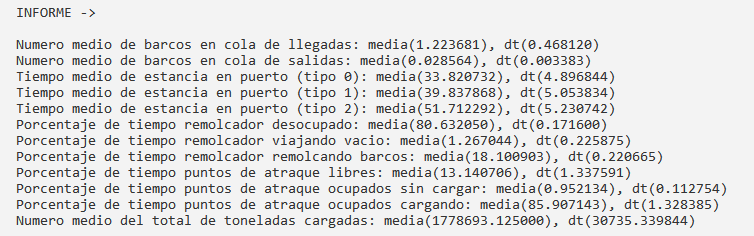
\includegraphics[scale=0.7]{img/puerto-mej1.png}
\caption{Simulación del puerto sin mejoras.}
\end{figure}
\begin{figure}[H]
\centering
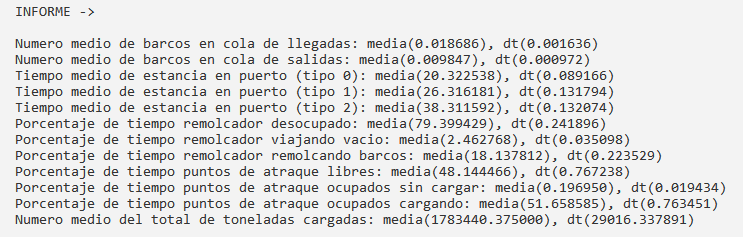
\includegraphics[scale=0.7]{img/puerto-mej2.png}
\caption{Simulación del puerto mejorado.}
\end{figure}

Podemos comprobar como estos cambios no solo producen una mejora de rendimiento del sistema, si no que también procuden una mejora de eficiencia. Vemos que para el modelo base, la
cantidad de crudo cargado es, en promedio, unos 10.000 kg menor que en el modelo mejorado. Por lo tanto, podemos concluir que tener un buen modelo de simulación nos puede servir
para determinar en que es preferible invertir o gastarse un dinero para mejorar alguna de las partes del sistema, ya que hemos visto que unas mejoras no son tan efectivas como otras
y que además podemos estimar cómo de buena puede ser (con kg de crudo en nuestro caso).



\chapter{Análisis de Salidas y Experimentación}

En este capítulo vamos a comparar y analizar empíricamente el modelo original y el modelo en el que el remolcador puede operar incluso cuando hay tormentas. Para ello vamos a
utilizar un script que ejecute los programas con 100 simulaciones y posteriormente, compare los resultados uno a uno y saquemos un porcentaje de veces en el que un sistema es
mejor que el otro.

El script está hecho en python, y se proporcionará también junto con la memoria y el resto de archivos. Como nos dice el guión, vamos a probarlo para 1, 5, 10, 25 y 50 simulaciones,
y vamos a analizar si es factible la mejora en función de estas. Veamos los resultados:

\begin{table}[H]
\centering
\begin{tabular}{c|c|c|c|c|c}
\textbf{Número simulaciones} & \textbf{1} & \textbf{5} & \textbf{10} & \textbf{25} & \textbf{50} \\ \hline
\textbf{NBCA\_A (\%)}        & 43         & 38         & 29          & 2           & 0           \\ \hline
\textbf{NBCA\_B (\%)}        & 57         & 62         & 71          & 98          & 100         \\
\end{tabular}
\end{table}


Como podemos ver, a medida que hacemos más ejecuciones, aumenta el porcentaje del sistema con el remolcador mejorado. Esto se debe a que con pocas simulaciones se cometen más
errores, sin embargo, cuando lo hacemos con 25 o 50, se ve claramente como el modelo mejorado obtiene mejores resultados que el que no lo está.

A continuación, vamos a probar a compara el sistema original con el del remolcador más rápido, pero vulnerable a las tormentas. La forma de proceder va a ser la misma que la
anterior, pero en este caso con el nuevo programa. Estos son los resultados que hemos obtenido:

\begin{table}[H]
\centering
\begin{tabular}{c|c|c|c|c|c}
\textbf{Número simulaciones} & \textbf{1} & \textbf{5} & \textbf{10} & \textbf{25} & \textbf{50} \\ \hline
\textbf{NBCA\_A (\%)}        & 42         & 37         & 29          & 35          & 32          \\ \hline
\textbf{NBCA\_B (\%)}        & 58         & 63         & 71          & 65          & 68          \\
\end{tabular}
\end{table}

En este caso vemos cómo, si que generalmente este modelo es mejor que el original, pero sin una diferencia tan clara como en el anterior. También hay que tener en cuenta que con
nuestro script estamos analizando y comparando la media de barcos en la cola de llegadas, y como vimos en el punto 2.2.3, que un remolcador sea más rápido mejora sobre todo el
tiempo del remolcador viajando vacío. Si quisiésemos abarcar este problema también, tendremos que cambiar la variable a analizar, pero en caso de que lo único que queramos mejorar
sea el número medio de barcos en la cola de llegadas, estamos haciendo bien, ya que nos podemos ahorrar el dinero de realizar esta mejora.

\end{document}



